\documentclass[sigconf]{acmart}

\usepackage{graphicx}
\usepackage{mathtools}
\usepackage{framed}
\usepackage{cleveref}
\usepackage{hyperref}


\copyrightyear{2019}
\acmYear{2019}
\setcopyright{acmlicensed}
\acmConference[HPDC '19]{HPDC '19: International ACM Symposium on High-Performance Parallel and Distributed Computing}{June 24--28, 2019}{Phoenix, AZ}


\begin{document}
\title[Projecting Globel Filesystems into Local Containers.]{Projecting Global Filesystems into Local Containers for High-throughput Computing on HPC Resources}

\if 0

Abstract

Intro
- CVMFS & HEP applications
- NERSC/HPC resources
- mismatch, new requirements on HPC

Background and Challenges
- CVMFS requirements
- no FUSE, sudo, etc. on HPC
- Frequent updates to CMVFS
- need for past versions and present
- version consistency issues/mismatch with shared filesystem semantics
- DVMFS

-------------------

Identifying Dependencies
- tracing vs. static analysis
- represent deps. as a set of files -> equivalence between the two approaches
- possibility to include more than requested
- WLCG as testbed for tracing
- overhead of tracing
- sampling ratio for live applications

Projecting a Global FS
- projections vs. images
- SquashFS images vs. Docker, ...
- Shrinkwrap
- quantify image size vs. projection size
- data, metadata, cache costs
- creation costs

--------------------

Managing CVMFS Containers at an HPC Site
- multiple snapshots at different versions
- cost of large number of container images (storage, distribution, etc.)
- extreme cases: massive NERSC image vs. loads of tiny containers
- possibility of replacing an image with an augmented version to serve 2 apps
- tradeoffs in space, creation time, etc.
- online problem: create vs. augment

---------------------

PoC Implementation
- consider (path, ID) to deal with versions
- Jacard distance metric
- group images with common parts
- fast to (approximately) compute
- putting too many disjoint pieces in an image pushes it farther and farther away
- LRU to clean up

Evaluation
- sample workloads
- image vs. projection vs. cache size
- space savings
- image re-use
- construction time
- choice of alpha

----------------------

Conclusion

\fi

\author{Tim Shaffer}
\email{tshaffe1@nd.edu}
\orcid{}
\affiliation{%
  \institution{University of Notre Dame}
  \city{Notre Dame}
  \state{Indiana}
  \postcode{46556}
}
  
\author{Nicholas Hazekamp}
\email{nhazekam@nd.edu}
\orcid{}
\affiliation{%
  \institution{University of Notre Dame}
  \city{Notre Dame}
  \state{Indiana}
  \postcode{46556}
}

\author{Jakob Blomer}
\email{jblomer@cern.ch}
\orcid{}
\affiliation{%
  \institution{CERN}
  \city{Geneva}
  \country{Switzerland}
}

\author{Douglas Thain}
\email{dthain@nd.edu}
\orcid{}
\affiliation{%
  \institution{University of Notre Dame}
  \city{Notre Dame}
  \state{Indiana}
  \postcode{46556}
}  


\renewcommand{\shortauthors}{Shaffer et al.}



\begin{abstract}
Scientific applications often depend on large, complex software repositories containing libraries, tools, and frameworks in multiple versions and platforms to support many researchers.
As a practical necessity, software repos are most commonly distributed via shared or global filesystems.
In moving existing research to HPC environments, however,
scientists must work around restrictions that can interfere with global software delivery methods.
To illustrate these challenges,
we examine CVMFS, the CernVM File System.
CVMFS is a global, distributed filesystem that provides read-only access to experiment software and configurations for high energy physics research at CERN.
CVMFS requires a number of network and OS configurations that are incompatible with a restrictive HPC environment.
In this work, we introduce a set of tools and procedures for \emph{projecting} the global filesystem (or parts thereof) into local container images suitable for HPC sites.
As part of our evaluation,
we found that using local approximations of a global filesystem tends to introduce problems of its own in terms of compute and storage overhead.
We thus examined several declarative and profiling-based approaches to creating more fine-grained projections to fit application requirements,
and propose a strategy for efficiently managing these projected container images at an HPC site.
Using our projection tools and image management strategy,
we implemented a proof-of-concept submission system for running existing HEP analysis tasks in an HPC environment.
\end{abstract}


%
% The CCSXML code is generated by the tool at http://dl.acm.org/ccs.cfm.
% Please copy and paste the code.
%

%
% Keywords. The author(s) should pick words that accurately describe the work being
% presented. Separate the keywords with commas.
\keywords{global filesystem}


\maketitle

\section{Introduction}

Scientific research has a large and rapidly growing need for computation.
Researchers have a number of options at their disposal to meet those needs,
including campus-local or organization-local resources,
cloud providers,
grid computing,
and large HPC sites.
Moving applications between these classes of resources can present problems,
as the assumptions made during development may no longer hold.
For example, organization-local resources and some grid sites commonly provide access to shared filesystems at each compute node.
In addition, there is some flexibility in system configuration to support an organization's primary research activity.
A new computing environment may be much less open to changes for a specific application,
especially large, multi-tenant resources such as HPC sites.
In these cases, it is left to scientists to adapt their application software to the available resources.

Many of our research collaborators have experienced significant frustration in preparing an existing scientific application to run on a new type of resource.
As a concrete example for this work,
we consider the challenges in running simulation and analysis workloads at CERN on HPC sites.
These applications assume several pieces of infrastructure to be in place and require some configuration and customization to the compute environment.
This is not an issue when running on Worldwide LHC Computing Grid~(WLCG),
which is a dedicated resource built to meet CERN's substantial computing needs.
The WLCG currently satisfies most of the computational needs of the LHC experiments at CERN.
With the upcoming high luminosity upgrades to the LHC,
the computational resources needed will will increase by at least an order of magnitude by 2026,
% On CERN's page it estimate 50-100X need, argonne had a report that was 10-20X
prompting researchers to turn to available high performance computing (HPC) resources to meet demand.
%In contrast with the WLCG's single slot submissions,
%HPC applications typically consist of parallel jobs using several cores up to a full machine for each submission.

Most HPC systems, however, have site-specific configuration and security requirements.
These can take the form of limited network availability at computation nodes,
limited container support,
and restricted access to privileged system features (such as FUSE support).
These new restrictions present challenges when porting existing scientific applications,
which expect required software to be readily available,
make a number of assumptions about how the system should be configured,
and may not be designed with tasks such as converting between image and container formats in mind.

In the case of the simulation and analysis workloads at CERN,
unrestricted network access and FUSE support are critical for providing global filesystem access.
Nearly all research software used at CERN assumes the availability of the CernVM File System (CVMFS),
a distributed global filesystem built for distributing software and configuration data.
CMVFS provides a read-only, distributed file system using HTTP for network transport and extensive local
caching to rapidly distribute updates in software across the WLCG.
Dependence on CVMFS to distribute experiment software currently makes it impossible to take advantage of many HPC sites.
CVMFS requires unrestricted network access and is implemented as a FUSE module,
both of which sites often disallow for security and management reasons.

Some sites, such as NERSC,
have attempted workarounds for providing CVMFS,
such as creating large images several terabytes in size that contain all of the software stored in CVMFS or
maintaining local mirrors of CVMFS available via site-local shared filesystems.
However, both of these existing solutions require 
hours to days of attention from system administrators to deploy or update,
which leads to lag between the available software and the current version.
Additionally for systems that utilize large container images, large amounts of storage are needed to maintain different versions.

Since each LHC experiment job uses 
only a relatively small portion of CVMFS,
a more fine-grained approach to preparing container images would reduce the time spent creating images and allow for more precise control of the software versions in use.
This could also reduce the storage required at each worker node and the network bandwidth spent transferring images.
It is often possible to determine dependencies for particular applications statically by examining submission commands, setup scripts, etc.
This approach, while reliable, tends to be labor-intensive and tied to specific experiments and software stacks.
We therefore modified the reference implementation of CVMFS to allow us to capture the filesystem interactions of live HEP applications.
Using live tracing and static analysis,
we are able to determine exactly which parts of the \texttt{/cvmfs} file system tree CVMFS must be included in a container image for a particular job.
We developed a tool, Shrinkwrap, that can efficiently \emph{project} CVMFS (or a subset thereof) at a particular version into a traditional filesystem.
Such a \emph{projection} of CVMFS is suitable for inclusion in a static container image that does not depend on FUSE or network access.

While working with projected container images and Shrinkwrap,
we found that the cost of creating, distributing, and storing customized images for a large number of jobs and users creates unexpected challenges as well.
Shrinkwrap is designed to efficiently manage projections by deduplicating data in the filesystem.
Disk images, however, must contain complete copies of all included data.
The na\"{i}ve approach of creating a projection of CVMFS for each application results in frequent duplication of data and significant overhead in terms of computation and bandwidth.
Depending on the granularity of the projection,
image creation time can easily exceed individual job's actual compute time.
The alternative extreme, i.e.\ building a single large image that satisfies the requirements of all applications,
forces all jobs to use the same repository revision,
which can result in incompatibilities across applications.
Updates to the repository or changes in applications and requirements can again result in large amounts of overhead due to frequently creating, transferring, and storing these very large images.

Observing that jobs frequently have significant overlap in dependencies,
we designed a system to more efficiently manage container images on job submission.
First, we defined a metric for determining the similarity between projections.
This gives the possibility of identifying existing container images that could be re-used to fulfill a new request.
We also determined that in some cases,
it is less expensive to augment an existing, similar projection to allow a single container image to support multiple distinct applications.
We bring these tools together as a proof-of-concept submission system for making online decisions about whether to create, reuse, or augment container images to efficiently support high-throughput HEP jobs on HPC resources. 

Compared to existing solutions,
Shrinkwrap created more compact projections than traditional methods such as rsync copies,
and allowed for more efficient updates to existing projections.
Based on the existing projects to produce static CVMFS container images and traces of benchmark applications,
we examined the sizes and structures of several projected container images.
Based on these properties,
we simulated the behavior of our image management system over a large number of job submissions.
We found that our approach can effectively manage the container images for a continuous stream of submissions with varying software dependencies and versions with less storage overhead than creating a new image per application.
In addition, our results show that applications can still take advantage of precise dependency and version specifications to reduce image creation and transfer overhead compared to working with large/complete mirrored copies of CVMFS.

\section{Background and Challenges}

\subsection{CVMFS}
The CernVM File System (CVMFS) is a globally distributed filesystem designed for providing efficient,
read-only access to scientific software.
CVMFS is primarily used for distribution of High Energy Physics (HEP) software used as part of the Large Hadron Collider (LHC) at CERN.
Researchers at CERN use CVMFS as the primary means of distributing the analysis and simulation software they develop to the Worldwide LHC Computing Grid (WLCG).

Each WLCG site commits to providing some fixed amount of computational resources for analyzing particle collision events and running simulations.
Worker nodes at each site must be configured to mount CVMFS as a prerequisite to performing any computational tasks.
Since CVMFS is implemented as a FUSE module,
WLCG sites are expected to support FUSE on their worker nodes.
CVMFS also relies on global configuration files,
requiring administrative involvement in preparing worker nodes for WLCG jobs.
In addition, sites generally provision some infrastructure to support CVMFS,
such as caching proxies to reduce load created by local workers on publicly accessible filesystem servers.

As a result, it is difficult to contribute computational resources toward the LHC experiments without making some site-wide provisioning and configuration changes.
This is not an issue for the WLCG sites,
as they provide dedicated computing resources and can customize their setups to meet the requirements of CVMFS.
For a professor attempting to harness a campus cluster,
on the other hand, these requirements present a serious barrier.
Parrot, a debugging tool and personal filesystem developed at the University of Notre Dame,
can be used in cases where privilege on the worker nodes is limited and FUSE is not available but still requires unrestricted network access.
For computing at scale, it is important to provide a caching proxy as well,
which is likely to require assistance from administrators.

\subsection{HPC}

With the rapidly increasing demands of the LHC experiments at CERN,
HPC resources are an appealing source of computing power to supplement the WLCG.
Leadership class machines such as Summit (?) will by themselves be able to perform a substantial portion of the work of the entire WLCG today.
Use of national-scale HPC resources across the United States and Europe such as XXX, YYY, Piz Daint at the Swiss CSCS HPC center could be key in meeting the computational demands following the LHC's high-luminosity upgrade.

Unfortunately, HPC sites are generally more restrictive than the previously mentioned campus resources.
In addition to limited privilege on workers and lack of FUSE support,
HPC sites often impose restrictions on network activity,
including outbound firewalls preventing access to CVMFS.

The US collaboration of the ATLAS project is currently taking advantage of computing resources at various supercomputers in the United States including Cori at NERSC.
For the deployment of their software the \texttt{uncvmfs} utility is used to unpack entire CVMFS repositories into standalone images (usually in ext4 or squashfs format) which in turn can be used to build Shifter or Singularity images.
While these images can very well be scaled out onto a large number of nodes inside the NERSC infrastructure,
the image build process takes around 24 hours which makes it difficult to deploy up-to-date versions of the software on a regular basis.
As these images contain complete copies of everything in CVMFS,
each takes on the order of terabytes,
necessitating careful storage management.
In addition, the process requires administrators for image creation, deployment, and cleanup.
Currently, this approach is used in production on the ATLAS and CMS experiments.
As additional experiments want to take advantage of the resources at NERSC,
the administrative burden of managing multiple CVMFS images on multiple software versions increases accordingly.
For the experiments to use the same images (saving time and cost at NERSC),
multiple groups would have to come to agreement about a single common set of software versions to use and adjust their pipelines elsewhere.
Both solutions introduce new inconveniences and administrative burden.

More broadly, the use of static, manually managed container images breaks user assumptions about the operation of CVMFS.
When running jobs using CVMFS,
researchers can specify the version of each repo to use,
allowing precise control over software and dependencies.
Each experiment has its own policies and procedures for choosing a software version;
some may use bleeding-edge analysis software or another experiment may prefer older, stable versions.
CVMFS is able to provide multiple customized views of the global filesystem without incurring much additional cost.
CVMFS also supports some more exotic features,
such as symlink resolution controlled by environment variables.
CVMFS as a whole does not map well to the semantics of a traditional filesystem.
Projecting CVMFS into such a filesystem can capture at most a single, static version of a repo and must necessarily eliminate some features,
such as environment-based symlink resolution at runtime.

% https://indico.cern.ch/event/587955/contributions/2937411/attachments/1683156/2705423/WahidBhimji-CHEP18-NERSC.pdf
Another similar approach in use at NERSC is DVMFS.
Since creating static container images containing CVMFS is costly and difficult to customize,
DVMFS instead uses Cray DVS IO forwarders to mount a copy of CVMFS served over NFS.
This allows for less administrator involvement,
since the mirrored copy of CVMFS can be automatically updated on a regular basis.
After dealing with several implementation problems,
DVMFS is currently deployed at NERSC as an alternative to static images.
While this approach affords more flexibility in choice of repos and software versions,
it increases the job startup time and places additional requirements on the infrastructure.
To be usable in production, DVMFS requires a sufficient number of DVS servers to be provisioned.
DVMFS is nonetheless a viable solution as long as the costs of developing/maintaining the service and allocating infrastructure do not grow too high.

\section{Defining Application Dependencies}

While the entirety of CVMFS is fairly large,
a single application would never use every piece of data.
Rather than attempting to provide a complete copy of CVMFS locally,
which entails significant storage costs,
we could instead provide a limited subset of the complete filesystem that is sufficient for a particular job.
This approach is more in line with traditional software packaging practices,
where software is provided as needed in the form of RPM files or another similar format.
Working with software packages is simpler in that dependencies are explicitly specified in the package file or database.
With CVMFS, no such definitive specification exists.
This issue is common to shared/global filesystems,
since users expect the complete contents to be available on demand and so devote little time to explicitly defining dependencies and other requirements.

In the case of CVMFS,
building an accurate 
specification of the files, libraries, and packages
needed for each experiment is the first step toward creating usable container images.
Such file specifications can be used when 
projecting CVMFS into realized filesystems.
The correctness and storage overhead of the projected filesystem hinges on the clarity and accuracy of the file specification.
File specifications can be derived from several
different sources, such as 
usage traces, static analysis, or package listings.
The end goal of any of these methods is to 
create a comprehensive list of needed files and structure.
The nature of global filesystems flexible behavior
further extends file specifications by requiring
not just the files and structure, but also what
version/revision was used to verify the contents as well.

\subsection{Creation of Specification}
File specifications can be created several ways,
with the obvious option being handwritten.
However, this quickly becomes unfeasible with
even a moderate number of requirements.
This leaves the need for an automate method to create
specifications.
The first method is to create a sample trace for your
jobs. 
Creating a trace from a sample job allows 
for a listing of actual files used, which
can be more accurate than handwritten listings.
As these jobs are typically on the order of thousands
to millions of jobs, sampling a small subset
can provide good software coverage with little
additional overhead. % the computation is still used
The burden of creating these traces is
dependant on the method used,
which could be an LD\_PRELOAD library,
using Parrot to track used files, % I think parrot was mentioned previously
or building the tracing in to the application.
As we will see later, we chose application
level tracing as it provides more context
for the use.

The second automated method is to use static
analysis for discover requirements.
This would allow the application to be analyzed
prior to running to determine what packages are
linked.
Static analysis can be done at several levels,
each providing different levels of control 
and flexibility.
This could be more language specific in the 
form of following import lines in python or
include lines in C.
The alternative is to use repository specific 
methods for setting up the environment,
such as bash scripts for pointing to correct 
software versions, or 
analyzing SCRAM\cite{DBLP:journals/corr/cs-OH-0306014} lines
to determine the configuration.
With either of these methods the issues
that arise come from bleeding edge or
experiment specific code that is not directly
handled by the configuration.
There is a significant mix between languages,
configurations methods, and software organization
practices even within a single repository,
which compounds the above issues in this method.

An combination of tracing and static analysis is the
use of package listings. 
Package listings provide a high level indication
of the software needed, and allow for 
flexibility on the specifying user about the
exact files needed.
Using high level packages provides a method
for handwritten/tuned specifications that 
include all aspects of the package.
The downside of using packages is that in
their flexible, forgiving specification
they can be bloated and include unnecessary
files and data.
Packages also require that there is consistent
software organization, which often differs
between repositories.

For the analysis and creation pipeline discussed
later in the paper, tracing was used to provide
the file specifications. 
Tracings flexibility between repositories
and more precises file inclusion allow
for a lean package that provides coverage for
an experiment.

\subsection{Trace Sampling}
Tracing is attractive as it provides a consistent 
behavior between experiments and use cases.
In addition, it is easier to automate and sample arbitrary applications without assistance from each user.
This allows the solution to port between applications
quickly without having to delve in to the applications
specific configuration.
As previously mentioned, there are several methods for
obtaining a trace from a file.

Tracing was implemented in the CVMFS software and
interacts via the FUSE interface.
The tracing utility has been implemented in a way that 
minimizes the overhead if the tracer is deactivated and 
also minimizes the measurable overhead in the FUSE calls for an activated tracer 
by delegating the actual log writing to a separate thread to avoid blocks 
during the accesses to CVMFS. 
In fact, for a deactivated tracer the entire overhead consists of 
a single inline if for a subset of the FUSE calls.
This allows the actual observed CVMFS usage to  be tracked
and then used for determining the file specification.

Despite assumption that both CVMFS and FUSE will be limited
on the HPC site, this methods was used as it is reasonable to
allow for sampling of these jobs on WLCG. 
WLCG provides the flexibility of using CVMFS and FUSE, without
having to implement or provision a separate tracing infrastructure
at each site.
Additionally, as many of these jobs would have originally been 
destine to run on WLCG, the sampling sizes are unlikely to 
create significant overhead.
Using CVMFS for the tracing allows CVMFS's just-in-time deployment
of files to patch the environment and give an accurate view without
the risk of missing files.


\subsection{Unique Consistency Requirements}
CVMFS differs from traditional POSIX filesystems in that previous versions of all content remain available.
A researcher may specify the precise revision under which an application is known to run.
Thus the same path may refer to two completely different files for a pair of applications.
This is beneficial from the standpoint of reliability and reproducibility,
but complicates the process of projection.
A file specification needs to include enough information
to establish the directory structure and verify the contents at a specific revision.
This can be done in several ways, 
such as computing the checksum of contents,
using global revision numbers, 
or running verification software.
Computed checksums provide a system agnostic approach
to verification by allowing the checksum to be computed
at specification and verified before use.
Computed checksums provide a
consistency guarantee to the byte level,
but are often expensive at runtime for large
production systems.
This approach is alleviated in systems such as 
Git and CVMFS as the contents' checksums are 
computed at ingestion into the repository.
This method relies on the underlying system computing
and providing this information for verification.

The use of a global revision number provides a quick reference
on the state of the repository at the highest level.
Global revision numbers can instantly verify the expected
contents, but does not give evidence of compatibility between
revisions.
As the revision number is global, any change to the repository
is reflected in a change to the revision number, which means 
some software is unchanged between revisions.
This method leaves much to be desired when using common stable
packages that change irregularly.

Aside from computing and checking the contents of the
repository or its files, it is possible to verify the
software using experiment computation.
This is a common method used to testing software
and works equally when the target software provides
coverage of the features used by the application.
The difficulty here is in providing tests that
behave consistently, verify if computation is
incorrect, and cover the desired features.
Though it is possible for the submitting user
to provide test with coverage, application
developers have a better grasp of it usage
and how to provide coverage in testing.
An additional method is to run the application
on a determined site for initial results and
compare in the future for verification, but
this relies on deterministic code which is 
not always the assumption in HEP computing.



\begin{table*}[t]
\begin{center}
\begin{tabular}{|c|r r r|r r r|}
\hline
CVMFS & & ls -lr & & & Shrinkwrap & \\
Repository & Total Size (MB) & inode Count & Time to walk & 
  Data Files & Deduplicated Data Files & Deduplicated Data (MB) \\ \hline
%alice-ocdb & 482,642,307,428 & 1,621,661 & 2:22 &
% 1,621,282 & 1,595 & 24,433,131,203\\
%alice & 3,980,875,747,986 & 27,322,350 & 51:53 & 
%  797,404 & 23,996,541 & 2,098,509,015,172\\
alice & 3,980,875 & 27,322,000 & 51:53 & 
  797,000 & 23,997,000 & 2,098,509\\
%atlas-condb & 719,548,941,240 & 11,781 & 0:04 &
%  10,940 & 229 & 471,492,086 \\
%atlas & 6,195,013,689,056 & 120,598,601 & 3:48:07 &
% 8,823,179 & 85,554,444 & 3,760,712,059,548 \\
atlas & 6,195,013 & 120,599,000 & 3:48:07 &
 8,823,000 & 85,554,000 & 3,760,712 \\
%boss & 120,048,527,315 & 2,418,025 & 4:18 &
% 256,061 & 1,868,192 & 72,301,955,666\\
boss & 120,048 & 2,418,000 & 4:18 &
 256,000 & 1,868,000 & 72,302\\
%cms & 581,789,406,847 & 26,224,567 & 1:07:30 &
% 18,667,178 & 101,448,867 & *2,242,658,825,701\\
cms & 581,789 & 26,225,000 & 1:07:30 &
 18,667,000 & 101,449,000 & *2,242,658\\
%geant4 & 297,571,283,648 & 7,128,024 & 10:36 &
% 323,280 & 6,219,891 & 68,381,969,660 \\
geant4 & 297,571 & 7,128,000 & 10:36 &
 323,000 & 6,220,000 & 68,382 \\
%grid & 30,642,826,259 & 714,235 & 1:17 &
% 141,622 & 583,923 & 18,804,003,040 \\
grid & 30,643 & 714,000 & 1:17 &
 142,000 & 584,000 & 18,804 \\
%lhcb & 2,134,893,079,440 & 33,736,802 & 1:01:26 &
% 10,032,339 & 20,406,235 & 368,070,277,634 \\
lhcb & 2,134,893 & 33,737,000 & 1:01:26 &
 10,032,000 & 20,406,000 & 368,070 \\
%na61 & 5,222,967,734 & 25,602 & 0:02 &
% 8,609 & 15,001 & 2,425,507,431 \\
na61 & 5,222 & 26,000 & 0:02 &
 9,000 & 15,000 & 2,426 \\
%sft & 3,996,527,275,237 & 128,608,792 & 4:17:58 &
% 6,821,699 & 63,210,139 & 2,016,609,810,573 \\ 
sft & 3,996,527 & 128,609,000 & 4:17:58 &
 6,822,000 & 63,210,000 & 2,016,610 \\ 
 \hline
\end{tabular}
\caption{CVMFS repository sizes.}
\label{tab:repo-sizes}
This table shows the size, number of inodes, and the amount
of duplicate data that is eliminated using CVMFS.
\end{center}
\end{table*}

\if 0
I AM NOT SURE WHICH WE WILL USE. WRAP THIS UP LATER.
\fi

\section{Realization of CVMFS Projection}

\subsection{Definition of Projection}

In the case of global filesystems,
every time the filesystem is used locally
the flexible global state has to be 
locked for that concrete use case.
In the case of CVMFS,
this includes specifying the date-time
or revision number of the repository.
This state is used to determine 
what the global filesystem's directory
structure and file contents are, 
allowing for future use of the same state.
CVMFS is able to flexibly move
between these revisions using the FUSE module
to determine the structure and files and
relies on HTTP to pull any missing files.
However, with neither the HTTP access or
FUSE permissions, a method is needed to 
create and track realizations of this
state for future use.

We call these realizations of the global filesystem
projections.
A projection is a concrete filesystem image that can be
mounted, loaded, or copied into an existing system.
Projections can then be used to run experiments
and analysis using the global filesystem without
the previously mentioned permissions.
Projections have been used with CVMFS before,
in the form of unCVMFS and rsync.
UnCVMFS is a utility that projects an entire
CVMFS repository, at a set revision, into the local
filesystem. 
UnCVMFS utilizes CVMFS's data/file separation
to deduplicate the underlying data, but requires
entire repositories to be projected.
When used with several repositories for large projects,
unCVMFS can easily consume 500GB for single projection.
As is often the case, different experiments/analyses 
require different revisions that may conflict.

Rsync allows for file lists to specify and download
subsets of CMVFS repositories, but because it
was designed for general filesystem synchronization
rsync flattens the files, introducing duplicate data.
This direct representation of the file tree also
excludes the possibility of shared data repositories
between different projections.

% Probably need to mention that many applications assume
% CVMFS software is installed/mounted at /cvmfs

\begin{figure}[h]
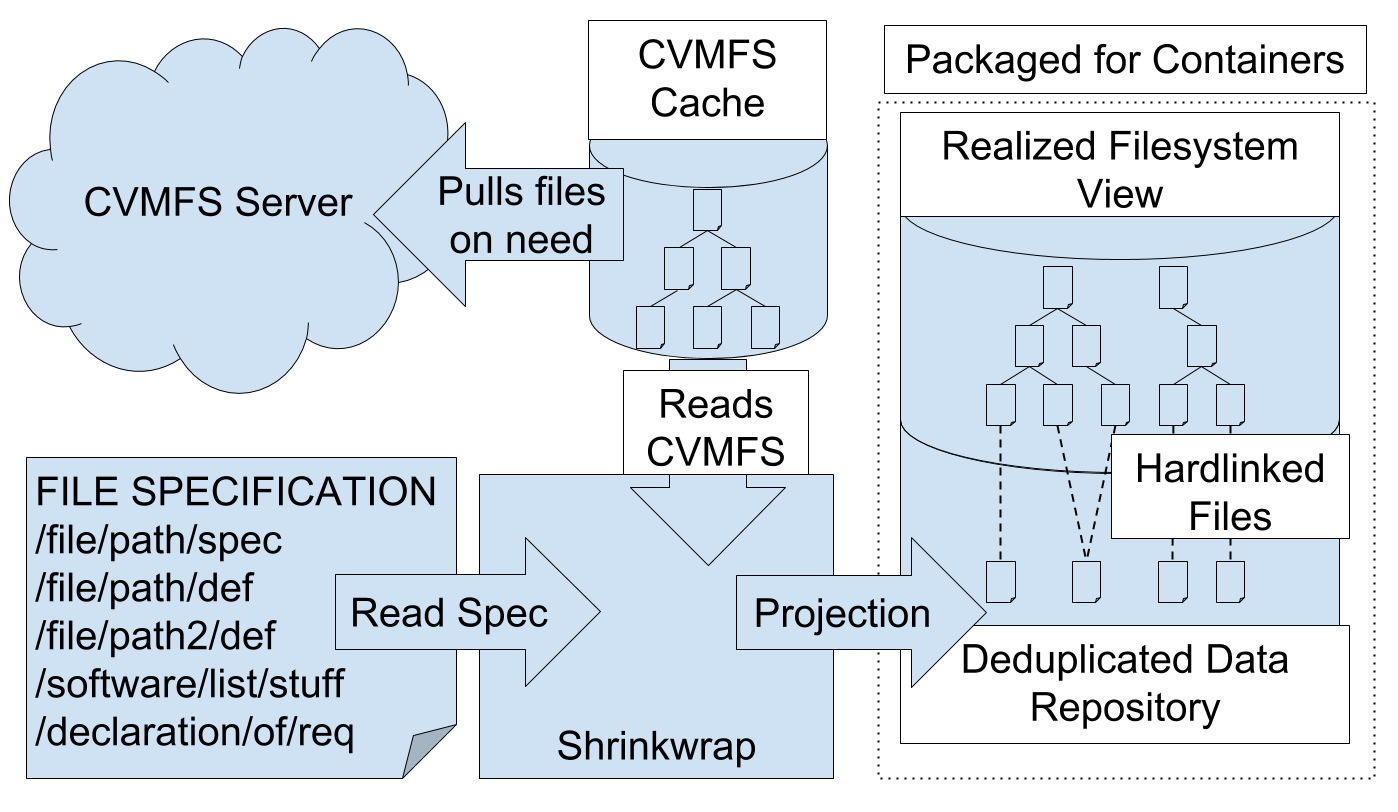
\includegraphics[width=\columnwidth]{drawings/shrinkwrap-structure.png}
\caption{Shrinkwrap Approach}
\label{figure:shrinkwrap-arch}
\end{figure}

We built the CVMFS Shrinkwrap utility,
a solution that leverages the best of both
unCVMFS and rsync.
Shrinkwrap uses the CVMFS's client interface to
create and update CVMFS projections.
Shrinkwrap uses a CVMFS configuration to specify the
revision of the repository, a file-specification list
to determine the repository subset to project, and
deduplicates the data in a user specified location.
Shrinkwrap can be configured to share the data
repository between several repositories and even
projections of the same repositories.
This allows for multiple realized projections
to coexist, with the desired projection
mounted for use.
In \Cref{figure:shrinkwrap-arch} you can see an outline
of the design of the Shrinkwrap utility.

These methods were compared to showcase Shrinkwraps
behavior and evaluate usage performance.
The first analysis compares all three methods pulling 
an entire repository, to allow comparision between the
three.
GRAPH OF DEDUPLICATED DATA/FULL REPO SIZE/TIME TO CREATE.
The second looks at the time to update existing repositories 
between verison.
GRAPH UPDATE TIME ON FULL REPO AND MAYBE SUB REPO(SUB REPO ONLY COMPARES RSYNC AND SHRINKWRAP)
The third looks at hosting several projection at once and
switching between them.
COMPARES RSYNC AND SHRINKWRAP. UNCVMFS CANT COMPETE.


\begin{figure}[h]
\caption{COMPARISON OF SHRINKWRAP unCMVFS and RSYNC}
\label{figure:projection-comp}
\end{figure}

\subsection{Packaging Projections}

All of the above methods describe utilize CVMFS
and rely on the internet connection to create
the projections.
A core assumption of this paper is that internet
access is limited at the compute nodes, so a method
is needed to transform and use these projections
for computation.
For this we looked at several methods for providing
these projections and compared using 
Container images (images specific to Docker, Singularity, ect.)
versus SquashFS images.
The goal is to find a flexible, compatible intermediate
format that allows projections to be moved between sites
and technologies.
For this purpose, Docker images, Singularity images, and 
SqaushFS are compared on their time to create,
storage requirements, and most importantly compatibility
with several used technologies, namely 
Docker, Singularity, and Shifter.

The first aspect is the creation of these images.
From a defined projection of a repository
what are the steps needed to create each of these image types.

When creating these images for analysis jobs its often the case that several
of these images may be created and used in the system.
Using Shrinkwrap to organize the repository data and projections,
the impact of an increasing number of images can be see in 
\Cref{figure:spec-size}.
This graph illustrates a new challenge that needs to be addressed.
As the number of experiments run and projections hosted by Shrinkwrap
increase. 
The raw number of images that need to be host increases to an unmanageable
size.
A solution is needed for how to manage these images and still
provide responsive execution of HEP analysis on HPC.

\subsection{Use Cases of Shrinkwrap}
%Here we illustrate several real world use cases.
%These use cases are being used as the existing solutions
%were not feasible and a new approach was needed.
%In analyzing these use cases we can see the beginnings of
%the problem outlined in the previous subsection.

\subsubsection{Atlas at NERSC}

We are currently discussing options to integrate our shrinkwrap utility into the HPC deployment processes of ATLAS as we believe that the proposed software solution can help to reduce the overhead of HPC software delivery significantly. On the one hand the actual uncvmfs export process can be optimized as the current export workflow loads the entire CVMFS repository in a first step and later on removes certain files in the exported image which were not in fact needed. This is something that can be entirely avoided through the definition of exclusion rules passed to the shrinkwrap utility.

On the other hand, we believe that an export client which relies on the libcvmfs library might reduce the total overhead and therefore improve the export performance in comparison to both uncvmfs and rsync (for uncvmfs this is something that we haven’t had yet the chance to evaluate in an experiment).
As a longer-term goal, it might be useful to start tracing ATLAS simulation workflows on a few machines to collect data that might allow further export optimizations in a later stage through automated specification building.

\subsubsection{Benchmarking Containers}
For benchmarking purposes, the CERN IT-Department is interested in a ``Benchmark in a Container'' solution which allows the distribution of standalone container images for system performance evaluations. For such benchmarks the IT-Department typically relies on simulation workflows provided by CERN's experiment collaborations. To execute these benchmarks in an easily portable and reproducible manner, it is of high interest to package these software workflows into containers. Since the workflows' software stacks are usually stored inside CVMFS repositories, this is a perfect use case for the shrinkwrap utility and its Docker injection functionality.

For the image export the workflow’s resource-needs would be examined through the CVMFS tracing feature in a first step. This would then result in a log containing detailed insights on the paths which were accessed by the benchmarking workload. In a second step we can then produce a specification based on the tracing log which will allow an easy, efficient export of the necessary files from CVMFS. Afterwards the Docker injector can be used to inject the exported files into a prepared benchmarking container stored in a registry. Later, the same utility can be used to update the current container to an up-to-date software version or — depending on the exact use case — the utility could even be integrated into a continuous deployment mechanism which produces new benchmarking containers on every software update.

\section{Managing Projections as a Site-wide Resource}

With static analysis and dynamic tracing of tasks,
we have methods to choose subsets of CVMFS to project to run specific tasks.
Users can collect this information themselves,
or tracing, too, could be handled automatically.
We have seen two approaches to this in section ??.
For applications already running on the WLCG,
it is also possible to instrument a fraction of runs to build a profile of the type of task.
Alternatively, we could integrate tracing with image creation by automatically running a small number of sample tasks on the WLCG or on dedicated bridge nodes and collecting traces as necessary.
These approaches give a fair amount of flexibility in determining accurate dependency information.
Based on this information,
we are interested in automatically providing suitable projections of CVMFS to users.

Shrinkwrap provides a mechinsm for projecting parts of CVMFS,
but is not by itself a complete solution as it does not integrate with job submission or manage images after creation.
In the case of a small number of manually created container images,
this is not a serious problem.
Administrators could manage a small collection of images in this case and adjust jobs to work with their setup.
Thus for integrating with the existing systems at NERSC,
Shrinkwrap alone might be sufficient.
To support CVMFS as a site-wide service with a potentially varied user base and workload,
a more automated solution
(e.g.\ a batch system plugin that can automatically prepare container images on job submission)
is required.
This both minimizes direct administrator burden and more closely approximates user experience on other resources like the WLCG.
Our first attempt at such a system,
described in the next sections,
took the simplest possible approach to image.
As we were developing this approach, however,
a number of issues in real-world usage led us to conculde that a somewhat more sophisticated solution was required.

\subsection{An initial approach}

The simplest approach for automatically projecting container images is to create a suitable image on each batch job submission.
Unfortunately, this solution is very wasteful of computing time and storage space.
Even a minimal image consisting of a precise set of required libraries and frameworks ranges in the tens of gigabytes,
depending on the application.
The full-repo images being tested at NERSC are multiple terabytes in size and take the majority of a day to create.
In addition, image creation must be completed before any actual processing occurs,
i.e.\ there is no way to start with a partial image that supports the first steps of a pipeline and finish building the image as the pipeline runs.
There is also the cost of transferring and storing freshly created images on any nodes that will use them,
further delaying job dispatch and increasing load on the network and storage infrastructure.

The disk I/O alone required to create even a targeted image is likely to take more time than a single simulation or analysis job.
Thus a simple performance improvement is to re-use previously created container images for multiple jobs.
A single experiment submitting computational tasks is likely to request the same projection of CVMFS,
at least for jobs submitted around the same time.
It is straightforward to check for exact equality between projections as long as the system retains the set of files that went into their creation.
Note that it is important to retain both the paths and the hash of the file contents used in images.
This ensures that multiple versions of the same file over time are recognized as distinct entities.
If there are few CVMFS users at a site,
this method could be sufficient.

After creating a set of static images,
the next step is to transfer them to local caches on the workers.
Worker nodes are assumed to have some fixed amount of storage available for caching images.
If the size of the ``working set'' of images is smaller than the node-local storage,
then each worker can keep a complete set of images.
While ideal, this case is not necessarily realistic beyond a few images.
With small/medium images in the tens-to-hundreds of gigabytes range,
maintining a complete set of projected CVMFS images at each worker requires substantial resource provisioning.
Thus it is important for workers be able to to cache only a subset of the available projected images.
There are numerous caching policies and options available,
but choice of worker cache strategy is not critically important for this application.
Since projections and images of CVMFS can be re-created on demand,
cache evictions might result in computation overhead but would not otherwise affect the functionality or correctness of the system.
In the absence of a compelling and site-specific reason,
a simple caching policy such as LRU would be sufficient.
As we will see in section ??,
LRU will also be an important piece of our final proposed approach.

Under this design,
on job submission the bridge machine first checks if the same projection had been requested before.
If so, it arranges to transfer its cached container image to worker nodes that lack that image locally.
If the bridge node does not have that projection built already,
it uses Shrinkwrap to create the requested projection,
then invokes mksquashfs to create the container image.
Once the bridge node places the newly created image in its cache,
the process proceeds as in the previous case.
The architecture of this initial approach is shown in figure ???.

%Node-local scratch storage is sufficient for temporarily caching these images.
%We also assumed that durable storage is available on the bridge machine for storing the data cache and projections associated with Shrinkwrap,
%as well as a cache of container images derived from these projections.
%Again, we chose LRU as a caching policy for our evaluation,
%though administrators would be free to experiment with different policies.

%Technologies like Docker currently operate this way (often to the chagrin of users and administrators doing scientific computing).

\subsection{Problems with the initial approach}

In developing our initial approach,
we found that a number of real-world usage patterns are poorly handled.
A small change to a projection,
such as adding a library or updating dependencies,
results in the creation of a second, unrelated image.
Even a small change such as removing an unnecessary documentation file results in a completely new container image.
This is a manageable nuisance when manually testing or developing a system,
but potentially results in problematic proliferation of images in a system managing images automatically and receiving updated specifications over time from tracing jobs.

In addition to unnecessary duplication for a single user/application,
there is also significant duplication across multiple users.
In the simulation and analysis pipelines at CERN,
a number of large components such as ROOT are used nearly universally.
These components provide basic functionality and infrastructure that each experiment's software stack builds upon.
Moreover, these same common infrastructure components must be included regardless of user or application.
Thus even if every user of the system only creates a single container image,
there is a duplicate copy of all such common infrastructure components for each user.
This is problematic if we would like to design a system that can support many users at a site.

These two sources of duplication tend to compound each other,
leading us to conclude that a more sophisticated approach is necessary to work with realistically-provisioned workers and system infrastructure.
These issues are fundamentally related to unnecessary duplication of data among container images.
The same types of issues motivate the use of dynamic libraries for everyday applications.
With statically linked executables,
each application includes a complete set of required libraries.
While very stable and reliable,
OS distributions prefer to use dynamic linking.
This allows applications to share a single copy of each library,
so that foundational components such as libc are not copied into every executable,
and so that updates and changes to the set of installed packages do not require rebuilding the entire system.
For this approach to work,
package maintainers must arrange all software packages in the system to ensure compatibility,
and the OS distribution must set policies for system organization, update procedures, etc.
Container images here function similarly to statically linked executables,
but since multiple complete OS distributions are stored within CVMFS,
and since we are dealing with multi-terabyte repos and entire frameworks and software stacks rather than individual OS libraries,
the scale involved is of course larger.
In the case of CVMFS, there is no notion of a ``package mainainer'' or central authority over all software.
Each experiment manages its own software repo as it chooses,
with some components and repos shared between multiple applications.
Since we would like to be able to automatically handle existing applications that are not designed with central management in mind,
we must instead look at other approaches for dealing with data duplication.

\subsection{Deduplicating Container Images}

The representation of projections as disk images is problematic for deduplicating data.
Internally, Shrinkwrap uses hard links to a common data store so that a single file is only stored once across all projections in the system.
On creating disk images, however,
these links are broken.
Each disk image must contain a complete copy of all data,
so that a file must be included (and take up space) in every image that includes it.
Docker's solution is to build container from layers of archives that can be reused.
Docker layers are explicitly defined when writing a Dockerfile.
With CVMFS, however, there is no existing layer-like organization or universal rule that could derive layers for existing applicaions.
Working with layers defined from the outset is also a poor fit if we would like to support partial, gradually improved information from traces.
We therefore desire some sort of deduplication that can be applied for existing applications to an assortment of container images after creation.

To develop a deduplication strategy,
we started with some observations about the projection and image properties.
For ``large'' images,
there is limited opportunity for deduplication.
Each large image is a fairly complete copy of a particular repo.
While there is bound to be some overlap between versions of the same repo,
an updated image will contain a large number of updated software components,
making a ``deduplicated'' between two versions significantly larger than either individually.
There are also likely to be some conflicts in the filesystem if software components re-use the same paths for different files between versions.
This case is akin to combining RHEL~6 and RHEL~7 in an attempt to save space.
While there are similarities between the two,
the significant changes and conflicts make this a poor strategy.
Thus for our strategy we would like to avoid ``deduplicating'' images that have large non-overlapping portions.

Likewise, there is little reason to attempt to deduplicate large images built from different repos.
Such images would have little to no overlap,
so the only benefit to combining the two would be reducing the number of images by one.
This comes at the cost of needlessly storing and transferring the unused half.
This case is akin to bundling a complete Debian installation alongside RHEL.
Our deduplication strategy should only take effect for images with significant overlap.

It is also undesirable to combine images of drastically different size.
As an example, suppose a user creates a small projection as a subset of a repo for running a specific application.
This small image overlaps completely with a large image of the whole repo,
and there is likely no conflict.
Automatically combining the large and small image, however,
can have unintended consequences.
Small, tailored images minimize transfer and storage overhead,
and can be important for operating at scale.
It is therefore unwise to surprise users by suddenly making their container images several orders of magnitude larger.
This is akin to distributing a library exclusively by placing it within a disk image of a Debian installation.
We would therefore like to attempt deduplication only for
\begin{itemize}
\item similarly-sized images.
\item with large overlap.
\item and with no conflicting paths.
\end{itemize}

\subsection{Quantifying Similarity between Projections}

Having set out the conditions under which to consider deduplicating projected images,
we are in a position to define a metric to quantify the similarity between images.
This would allow us to identify projections that are ``close'' (for some definition of close) as candidates for optimization.
We chose the Jaccard distance under appropriate choice of set elements as it conveniently satisfies the desired qualities set out above,
and is very well used and studied.
In our case, we must describe a container image as consisting of a set of (path, content hash) tuples.
CVMFS already stores files by the hashes of their contents,
so this information is readily available.
Considering both the file names and contents is important as CVMFS allows for updates to file contents over time.
We chose fine-grained tracking of file contents rather than simply recording the version of the CVMFS repo to afford additional opportunities for dedupliaction.
Since each update to a repo does not change the contets of every (or even the majority of) files,
data from multiple repo versions may well be able to coexist in a single container image.

For two sets $A$ and $B$,
the Jaccard distance $d_j$ is defined as follows.
\[
d_j(A, B) = 1 - \frac{|A \cap B|}{|A \cup B|} = \frac{|A \cup B| - |A \cap B|}{|A \cup B|}
\]
The Jaccard distance is a metric in the mathematical sense,
making many intitive assumptions about distance and relationships between elements mathematically sound.
For the purposes of comparisons,

For this application in particular,
the Jaccard distance captures several desirable properties of projections.
In the case of two projections that differ only by one file,
the Jaccard distance will be small.
Likewise for a par of projections with nothing in common,
the distance will be high.
And since the Jaccard distance is a proper metric,
related projections will tend to occur in clusters;
if two projections are both found to be extremely close to a third projection,
we can conclude that the two are themselves close by the triangle inequality.
Other choices of metric may well be viable,
but we found the Jaccard distance to be both well-studied and amenable to efficient approximate impelementation.
As described in section ??,
we used MinHash~\cite{minhash} as a constant-time approximation of the Jaccard metric as a first pass at selecting similar images.
Such an approximation is important in practice due to the sizes of the data involved;
metadata listings alone (not including any file data) consumed multiple gigibytes of storage in some of the container images we evaluated.

\subsection{Image Management as an Online Problem}

\begin{figure*}[t]
\centering
\fbox{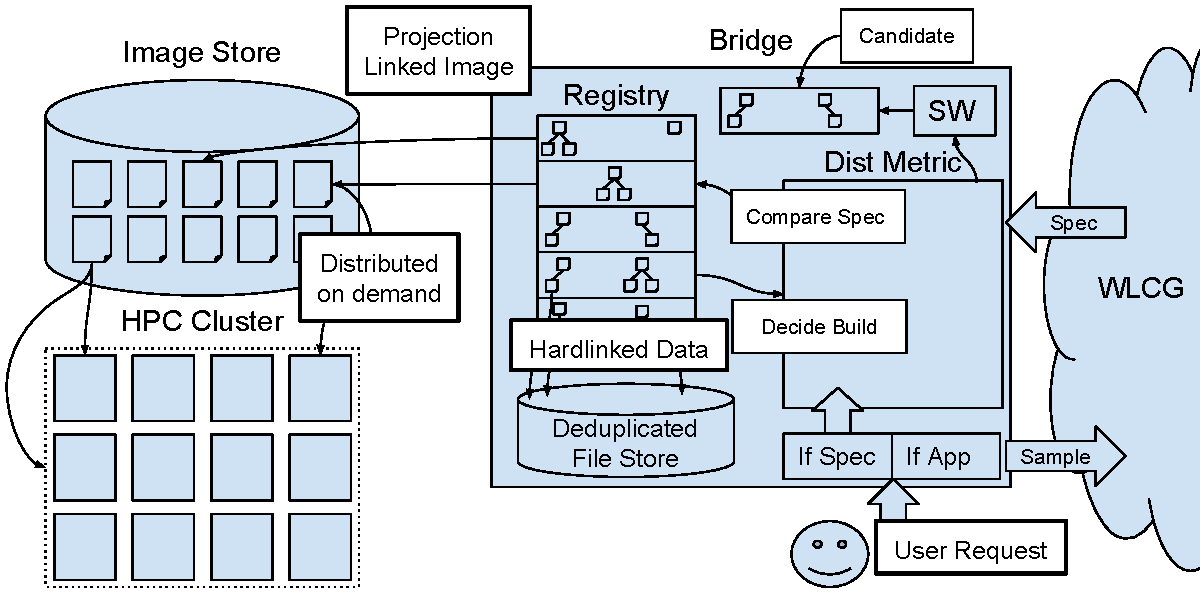
\includegraphics[width=0.95\textwidth]{drawings/system_architecture.pdf}}
\caption{Architecture of a Site-wide Image Management System}
\label{figure:sys-arch}
\end{figure*}

Combining the tools and techniques introduced so far,
we are now ready to address the central problem in managing projected images as a site-wide service.
Rather than relying on administrators to manually manage images,
we must define a method for making a decision online as to how to efficiently satisfy the dependency requirements for batch jobs.
Our method must be suitable for inclusion as part of the setup for batch job scheduling and must be efficient in terms of both computation time and storage space.
We will extend the initial implementation discussed in section ?? by tracking distances between projections and allowing existing images to be augmented rather than creating new ones for each request.
\Cref{figure:sys-arch} gives an overview of the structure of this system.

Upon receiving a request for a projection,
we first hash the new projection according to the MinHash algorithm.
We always store the hash values computed for every projection we build to allow for fast clustering.
Next, we use MinHash to approximate the Jaccard distance between the new projection and all projections previously built.
This computed distance can be cached to ensure that we estimate the distance between each pair of images only once.
Since comparisons using MinHash take constant time for a given probability bound independent of the size of the sets involved,
we can quickly identify cached projections that are similar to the new request.

To decide if two projections are ``close'',
we define the parameter $\alpha$ as the maximal Jaccard distance between closely related projections.
Since Jaccard distance is by definition between zero and one,
$\alpha$ must be in the same range.
This $\alpha$ parameter is something like the ``globbiness'' of the system.
Small choices of $\alpha$ requires that projections be extremely close before considering them for merging.
In the extreme case with $\alpha = 0$,
only \emph{identical} images will be considered close so no images will be merged.
This results in a larger number of independent images.
Choosing $\alpha$ to be larger makes it more likely for images to be considered similar and merged.
This results in more augmented images that serve multiple tasks.
In the extreme case of $\alpha = 1$,
\emph{every} pair of images is considered close and merged if possible.
This results in large container images that have accumulated many projections.
We explore tradeoffs when choosing $\alpha$ and give recommendations based on observed patterns of activity in section ??.

Having selected a set of candidate projections that are close enough to the new request,
we next check each in turn to find either a superset of the requested projection or one without version incompatibilities.
We first sort the list of candidate images by Jaccard distance.
This ensures that our system prioritizes candidates that are similar in size to the requested image.
In the case of finding a superset,
we can simply use the corresponding cached container image.
Presumably this superset was created by the merging process below,
so we are done.
Otherwise, we continue to look for a compatible projection
As discussed in section ??,
two projections are incompatible if they both include the same path but point to different data.
This situation can arise if for example a library in CVMFS is updated in place.
Old and new projections would include an identical filesystem path,
but the new version would have different contents.
This situation can arise in more subtle ways,
for example with symlinks controlled by environment variables.
Since projections of CVMFS must statically resolve such links,
incompatibilities can arise despite paths appearing compatible under CVMFS.
Any candidate projections that are incompatible with the new request are removed from further consideration.

If no compatible projections were found among the candidates,
we create a container image for the projection as requested and add it to the cache.
Otherwise, on finding a compatible cached projection the next step is to augment it with the contents of the new request.
We choose the first compatible image from the list of candidates for merging,
again prioritizing images that are similar in size and contents.
As previously discussed,
Shrinkwrap can update a projection that was previously created;
since we keep the projection used to generate each container image in the cache,
we can simply augment the selected projection with the new files from the request.
Next, we build a container image based on the newly updated projection.
The computational cost of this step could become high since we are creating larger combined projections.
Appropriate choice of $\alpha$, however,
bounds the distance between the combined projections such that the cost of creating the augmented container is arbitrarily close to cost of simply fulfilling the original request.
Since the augmented projection is the union of two different projections,
we can substitute it for both.
The container image for the augmented projection can replace the previous image,
so that the net increase in storage space comes only from the newly added files.
Since a single augmented image now serves two different batch job submissions,
we avoid making two copies of the common files and data.

One potential issue with this merging strategy is that there is no way to prevent poor merging decisions.
In the case of a one-off submission,
the system might merge an existing, frequently used image.
This is not problematic for the one-off job itself,
but increases overhead for subsequent jobs.
The original, frequently used image would increase in size with no additional benefit to other tasks.
Images might become ``bloated'' in this way,
accumulating infrequently used dependencies and increasing overhead indefinitely for future tasks.
The Jaccard distance metric gives a natural way to capture and quantify this effect.
As an image becomes bloated due to repeated merges,
its distance from every individual request increases.
After sufficient growth,
the image will become too far from any request to even be considered.
Without regular use,
the bloated image will eventually be removed in LRU order.
Choice of $\alpha$ allows an upper limit on the amount of useless bloat in images.

\section{Evaluation}

To evaluate the viability of our approach in automatically deduplicating a container image store,
we simulated the behavior of the system over time for a range of $\alpha$ values.
Choice of $\alpha$ is important here to ensure that common components can be detected and merged in container images,
and that old images or poor decisions are eventually removed from the system.
Choosing $\alpha$ too far in either direction will result in excessive storage overhead due to duplicated components,
or excessive compute and network overhead repeatedly merging largely unrelated images.
Our goal in this evaluation is therefore to choose $\alpha$ so as to minimize the storage and compute costs associated with maintaining a collection of images.

\subsection{Simulating Job Submissions}

The first step in simulating system behavior over time was generating synthetic requests for images.
We tested two schemes for generating image requests taking into account the properties of the software collections,
as well as recorded user activity patterns.
We also generated images via a uniform random scheme for comparison.
We consulted with the developers of CVMFS,
as well as HEP researchers at the University of Notre Dame collaborating with CERN to determine how current users interact with CVMFS.
Since CVMFS is not currently widely deployed on HPC resources,
the prospective user base for our container management system is limited.
We were, however, informed of some researchers and groups experimenting with static mirrors of CVMFS for container images,
including projects at NERSC and Stanford University,
with one of the setups available publicly at \url{https://github.com/wyang007/atlas-fat-container}.

Based on correspondence with researchers,
we made some general observations about the behaviors and requirements of applications we need to support.
First, there are some components such as ROOT that serve as common, foundational components to almost every other simulation and analysis stack.
These core components are often stored separately from the rest of the software collections available in CVMFS.
Second, there are shared components such as setup scripts, configuration files, and calibration or condition data (required to interpret readings from detectors) that are also nearly universally required but are more particular to a given experiment or group.
Finally, there is the collection of software maintained by each experiment.
Software collections may contain multiple copies of the same software for different architectures and versions.
A single analysis job does not use the majority of the available software.
There is some overlap among these categories of software,
for example some software components are widely enough used to be considered core components,
and usage and availability of components varies over time.

We use these observations about the structure and behavior of applications on CVMFS to build a simplified simulation taking into account dependency requirements for evaluating our container image management scheme.
For the purpose of simulation,
we assume that the requirements of a job are given as discrete components or collections of files.
While Shrinkwrap can operate at the granularity of individual files,
both static analysis and runtime tracing produce file collections to include.
We are intentionally somewhat vague here to allow for both explicitly defined software components and tracing outputs.
We examined the software collections available in the SFT repo and constructed a DAG of dependencies among the packages.
The currently available software collection in the SFT repo consists of NNN packages,
where a program or library typically provides packages for multiple versions and configurations.
When building a projection,
we recursively include dependencies of requested software.
This more closely approximates the structures of actual container images,
while still allowing for randomly selected package requests.
For each simulated image request,
we chose a random selection of packages (either uniform random selection or subject to the process below)
and then added the closure of the package dependencies.
This first image simulation scheme captures the structure inherent in the software collection,
in that packages in addition to those requested are automatically included so as to ensure a functional image.
The initial selection of packages,
however, is simply uniformly random.
This is not necessarily realistic, however,
so we next took usage patterns into account.

We assumed that certain components are included in most container images,
while other components are relatively rarely used.
While multiple versions and variations might exist,
these components have a very high likelihood of appearing in every container image.
These components correspond to the core components, setup scripts, calibration data, etc.\ described previously.
For the purposes of simulation,
we would like to see these components in a large proportion of jobs across all users and experiments.

We obtained CVMFS usage logs from frontend nodes at CERN,
which give rough usage frequencies of the packages in the SFT repo.
To generate simulated container requests,
we made random package selections subject to the observed distribution of package use.
Many packages in the repo were not observed being used at all,
so we added a small, non-zero probability of selecting packages lacking usage data.
We applied this technique in combination with the package dependency graph,
so that images contained a weighted random core selection along with any dependent packages.
This second image simulation scheme takes into account the dependency structure of the repo as well as usage patterns observed in the wild.

As a base for comparison,
we also generated simulated images consisting of packages chosen in a uniform random way.
To ensure that total size (or at least total number of packages)
is comparable to images generated by the previous two methods,
for this approach we started with an image request generated via the first scheme discussed
(uniform random core selection with dependencies added).
We considered only the number of software packages in the resulting image,
and then chose the same number of packages uniformly randomly from the entire repo,
ignoring usage information and package dependencies.
while images generated in this way are not particularly realistic,
they will be useful for evaluating image management schemes.
By comparing results with random images to those with the previous two image generation schemes,
we can compare the general case of containers as collections of arbitrary data to the specific focus of this work,
i.e.\ containers with selections of experimental software.

\subsection{Quantifying Image Management Costs}

The next step in evaluation is to define metrics describing the collection of cached containers.
Here we will define metrics in terms of discrete software components/packages to match the simulated streams,
but the same definitions would apply equally well at the granularity of individual files.
We will suppose that there is a collection of requested container images,
from either our simulated stream or from real user requests based on job analysis and/or dynamic tracing.
It is the responsibility of the image management system to provide a container image satisfying the requirements of each request.
Let the set $C$ be the union of all components in one or more requests.
$C$ provides a lower bound on the amount of space required to serve all requests at the same time.
If the storage space required to hold all of $C$ is greater than the total available storage,
then images serving new requests will requre removal of container image(s) for previous requests.
Since we have been considering image management as an online problem,
we cannot place an upper bound on the sizes of requests and thus require some caching policy
(in our case LRU) to ensure that $C$ is finite and fits available storage.
The large, full-repo images tested at NERSC correspond to single images containing all of $C$.
The image size is very large and any changes/updates are expensive both in terms of compute and bandwidth.
NERSC's approach does, however,
avoid duplication of data as there is a single image that serves all users and applications.

We thus define the multiset $A$ as the union (with repetition) of all components in a set of requested images.
If multiple images request the same component,
it will occur multiple times in $A$.
The size required to store $A$,
including all duplicated elements,
is the storage space that would be required if a separate image were created for each job request.
$A$ captures the amount of (potentially) unnecessary duplication in the collection of images.
The initial approach described in section ?? would have a storage cost of $A$.
Note that it is always the case that $|C| \leq |A|$,
and if $|C| = |A|$ then there are no common components among the requested container images.
While large, full-repo images provide the best storage efficiency, being based solely on $|C|$,
they are expensive and unweildy to use in practice.
The initial approach in section ?? is extremely simple and friendly to use in practice,
but its storage cost is determined by $A$.
Our goal, therefore, in evaluating our improved image management scheme detailed in section ?? is to achieve storage cost as close to $C$ as possible without excessive overhead in terms of compute and network bandwidth to keep the image collection up to date.
We define \emph{cache efficiency} as $|C| / |A|$ to quantify the amount of duplication in the system cache.
With poor cache efficiency,
the available storage for the system cache is wasted on repeated copies of the same data.
Improving cache efficiency allows for more more unique image data within the same storage space,
or equivalently allows the same set of job requests to be served efficiently from a smaller cache.

\subsection{Effect of $\alpha$ Threshold}

Using these metrics for cost and overhead,
we carried out an evaluation of our container image management scheme as follows.
First, we somewhat arbitrarily chose a storage limit of 1~TB for our simulated image cache.
This is not an unreasonable storage cost for an HPC site;
for the test setup in place at NERSC,
the full repo images already consume multiple terabytes per worker.
We experimented with different storage limits around the same order of magnitude,
but did not find marked differences in the behavioral trends observed below.
The important aspect is that some definite limit exist.
This does not take into account the storage used by Shrinkwrap,
which is automatically deduplicated,
nor does it take into account the metadata cost of creating projections.

The next step was to generate a synthetic stream of requests for container images.
These were generated using the procedure described previously.
To ensure that both the merging strategy and the caching policy come into play,
and to try to capture the steady state behavior of the system,
we continued the stream until the total amount of unique data handled was twice the storage capacity.
Equivalently, the request streams were long enough such that $C$ for the entire stream exceeded 2~TB.
We then tabulated the duplication ratio $d$ for the image cache,
as well as the total amount of data written over the course of the simulation.
Our goal is to minimize both duplication and data written,
which will be proportional to the compute and bandwidth cost of creating and updating container images.
We repeated this simulation W times and computed the averages and standard deviations of these metrics.
We repeated this procedure for a range of $\alpha$ thresholds in the range 0 to 1,
with the results shown in figure ??.

Looking at the results in figure ??,
we can see that small values of $\alpha$ result in the highest level of data duplication,
with $d$ decreasing as $\alpha$ increases.
Since $\alpha=0$ corresponds to the initial approach of creating a unique container image for each job submission,
we expect to see the highest level of duplication there.
Looking at the cost in terms of write activity,
we see that large values of $\alpha$ result in the most write I/O,
and thus compute and bandwidth overhead.
Since $\alpha=1$ allows all requests to be merged into a single large image,
we expect minimal duplication.
This configuration, however,
has substantial overhead for image creation and maintenance.
This is a real complaint from administrators at NERSC testing full-repo images.
The high cost of creation means that such large images can only be infrequently created or updated.


\section{Related Work}

\section{Conclusion}

\begin{figure*}
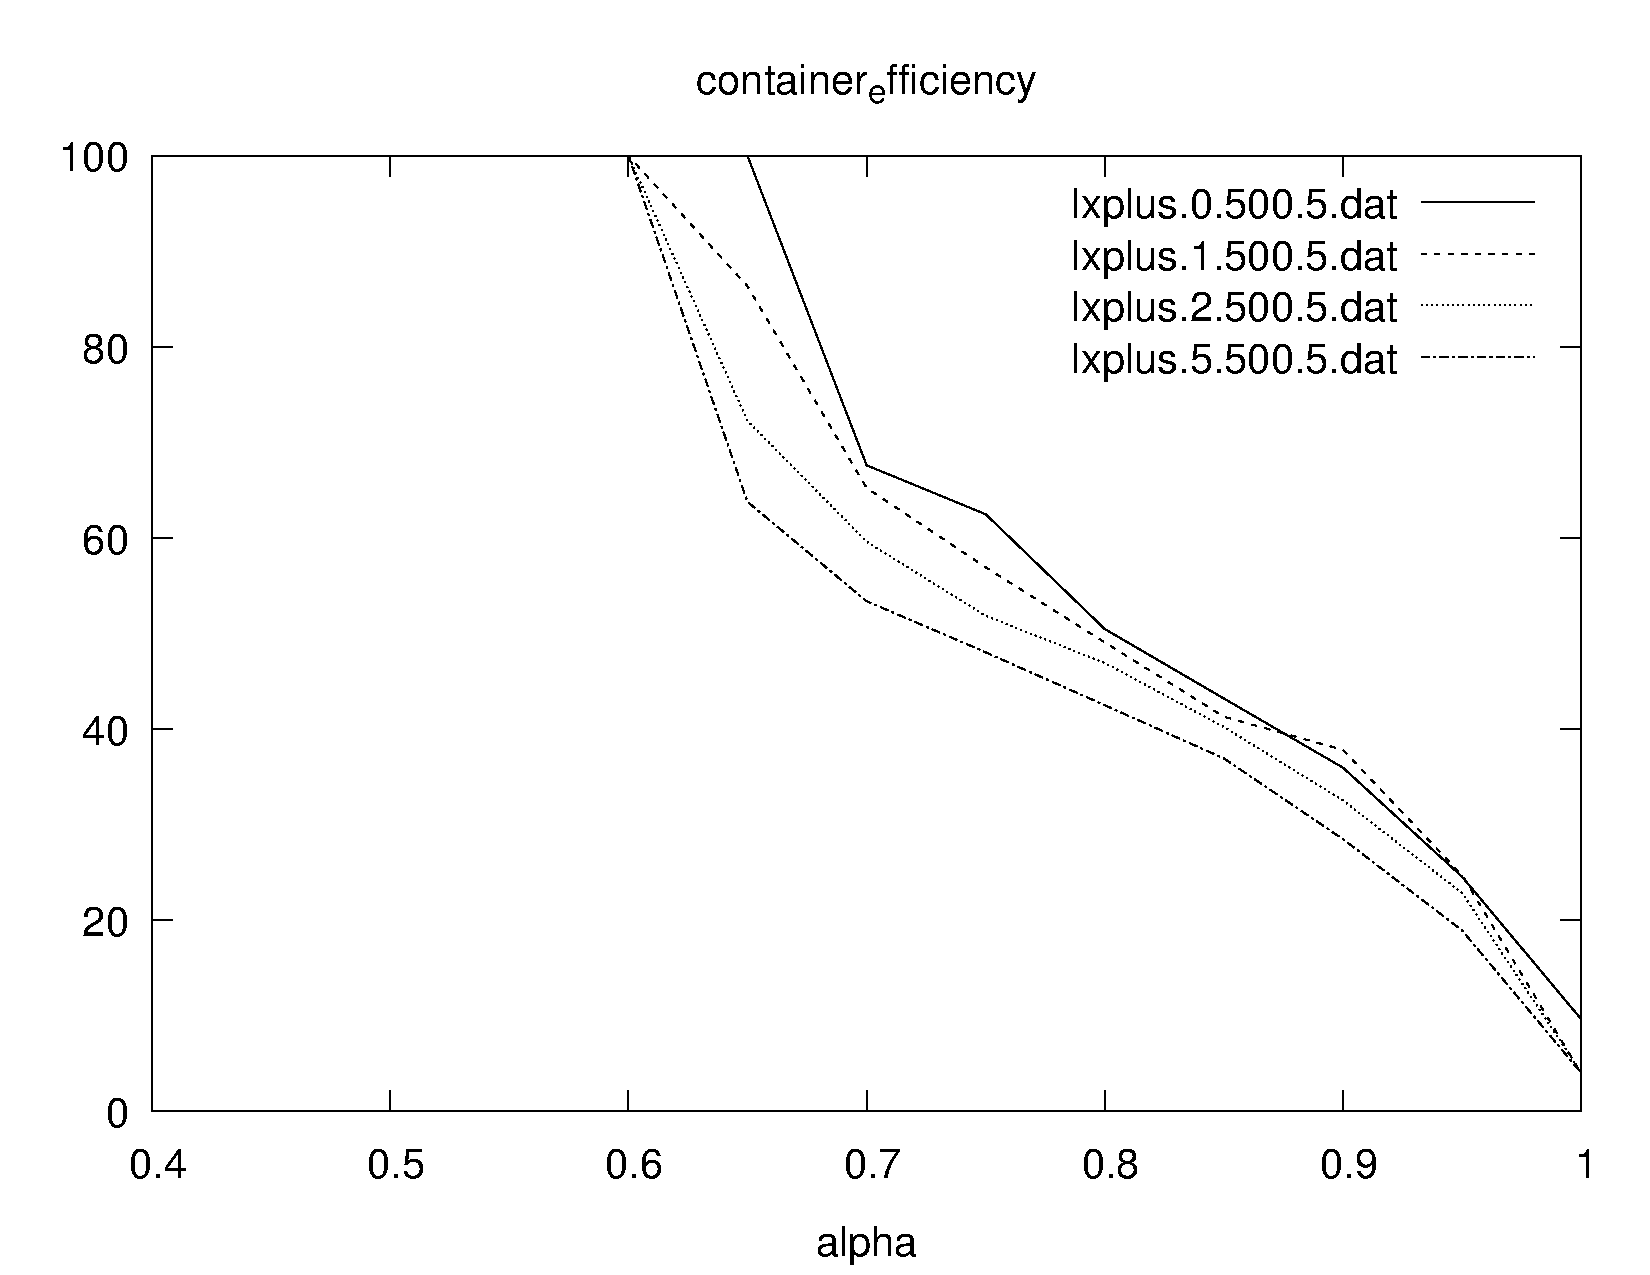
\includegraphics[width=0.48\linewidth]{curated/sensitivity/container_efficiency_cache_percent_plt.pdf}
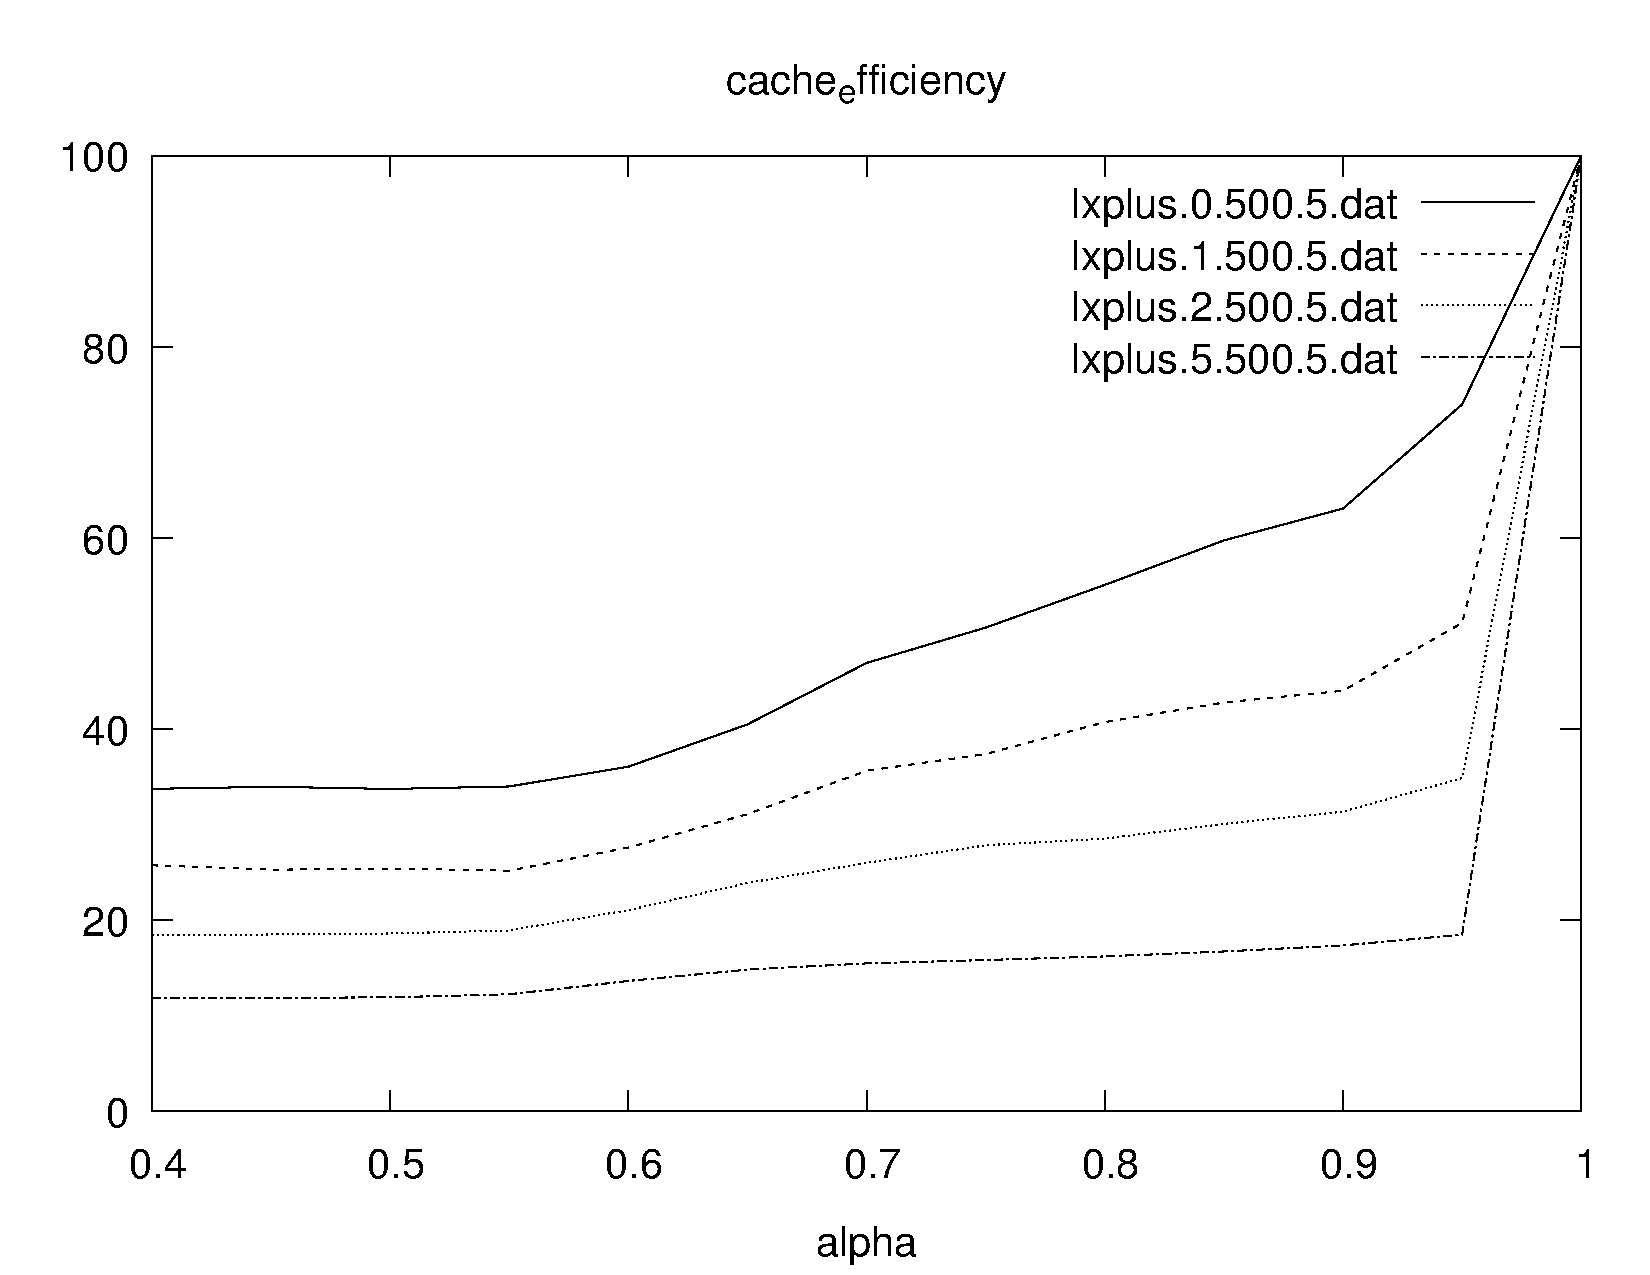
\includegraphics[width=0.48\linewidth]{curated/sensitivity/cache_efficiency_cache_percent_plt.pdf}
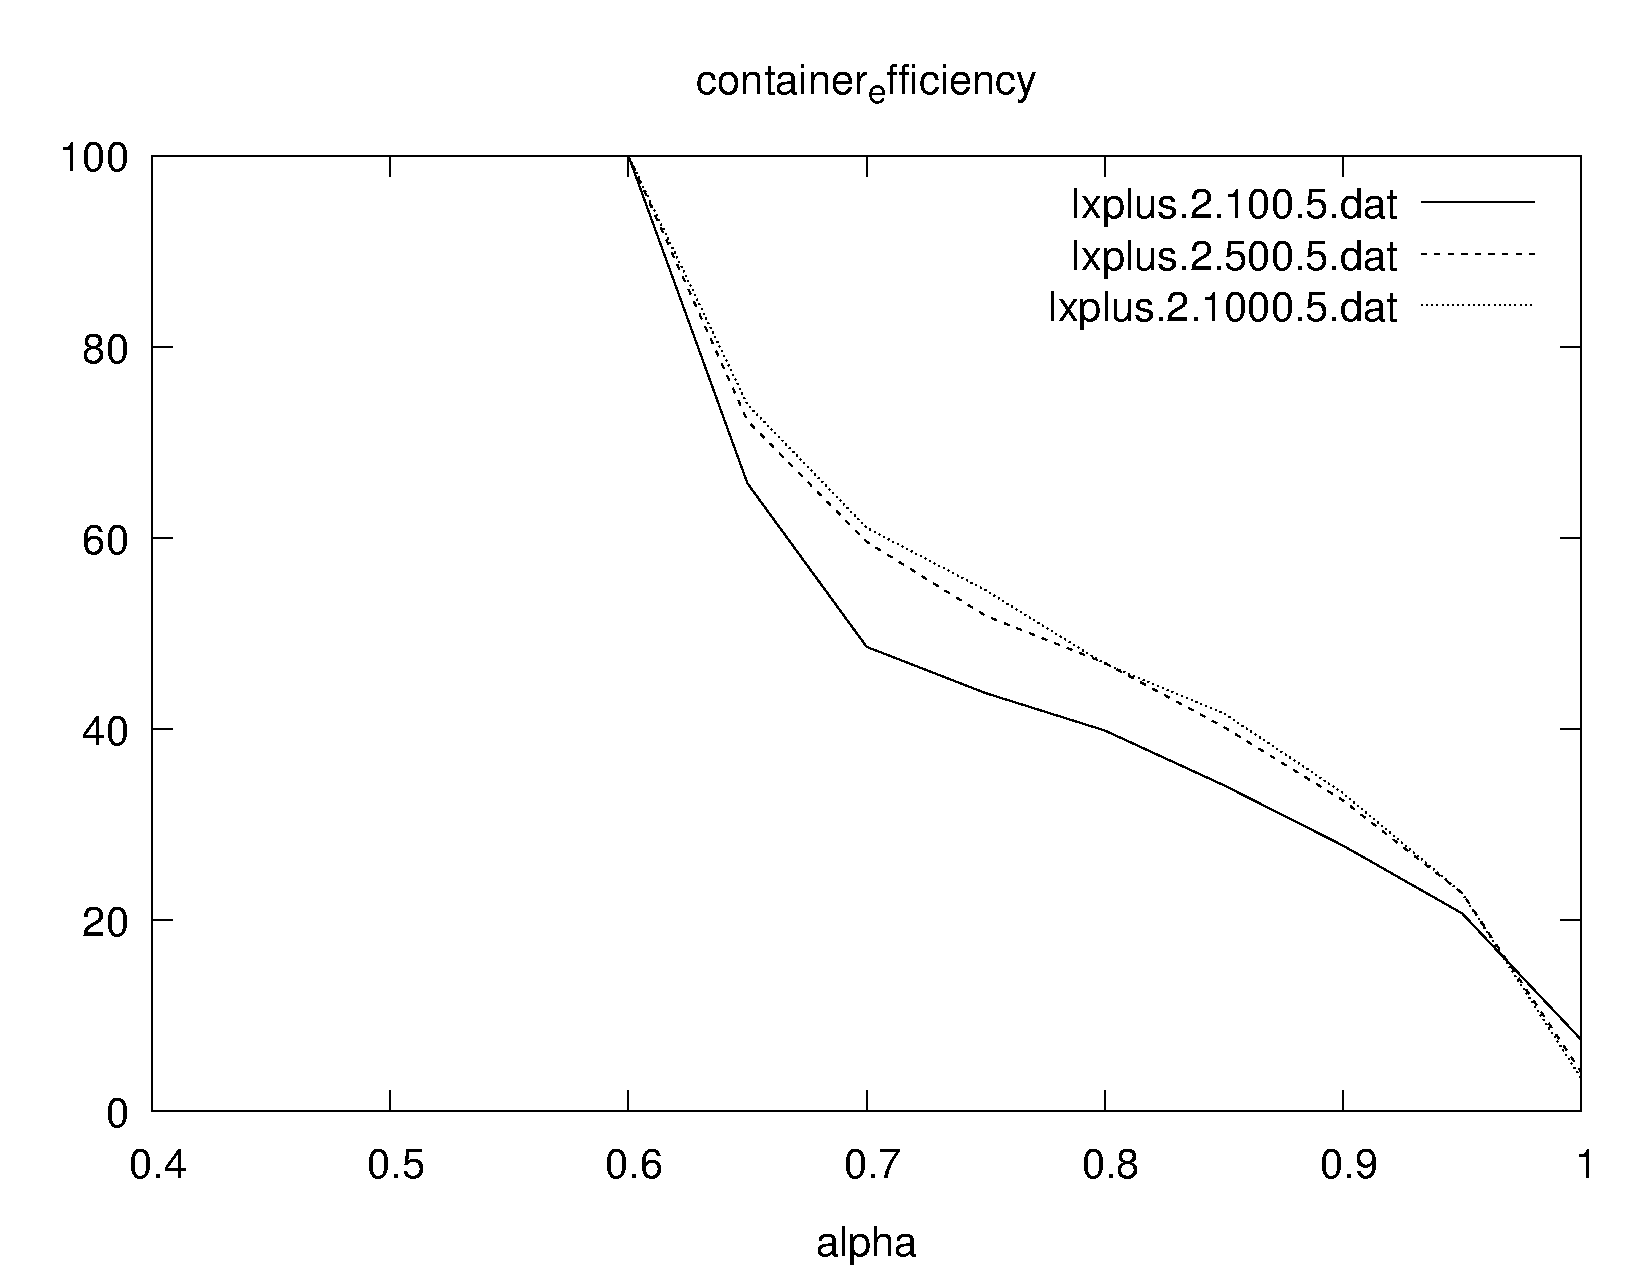
\includegraphics[width=0.48\linewidth]{curated/sensitivity/container_efficiency_request_percent_plt.pdf}
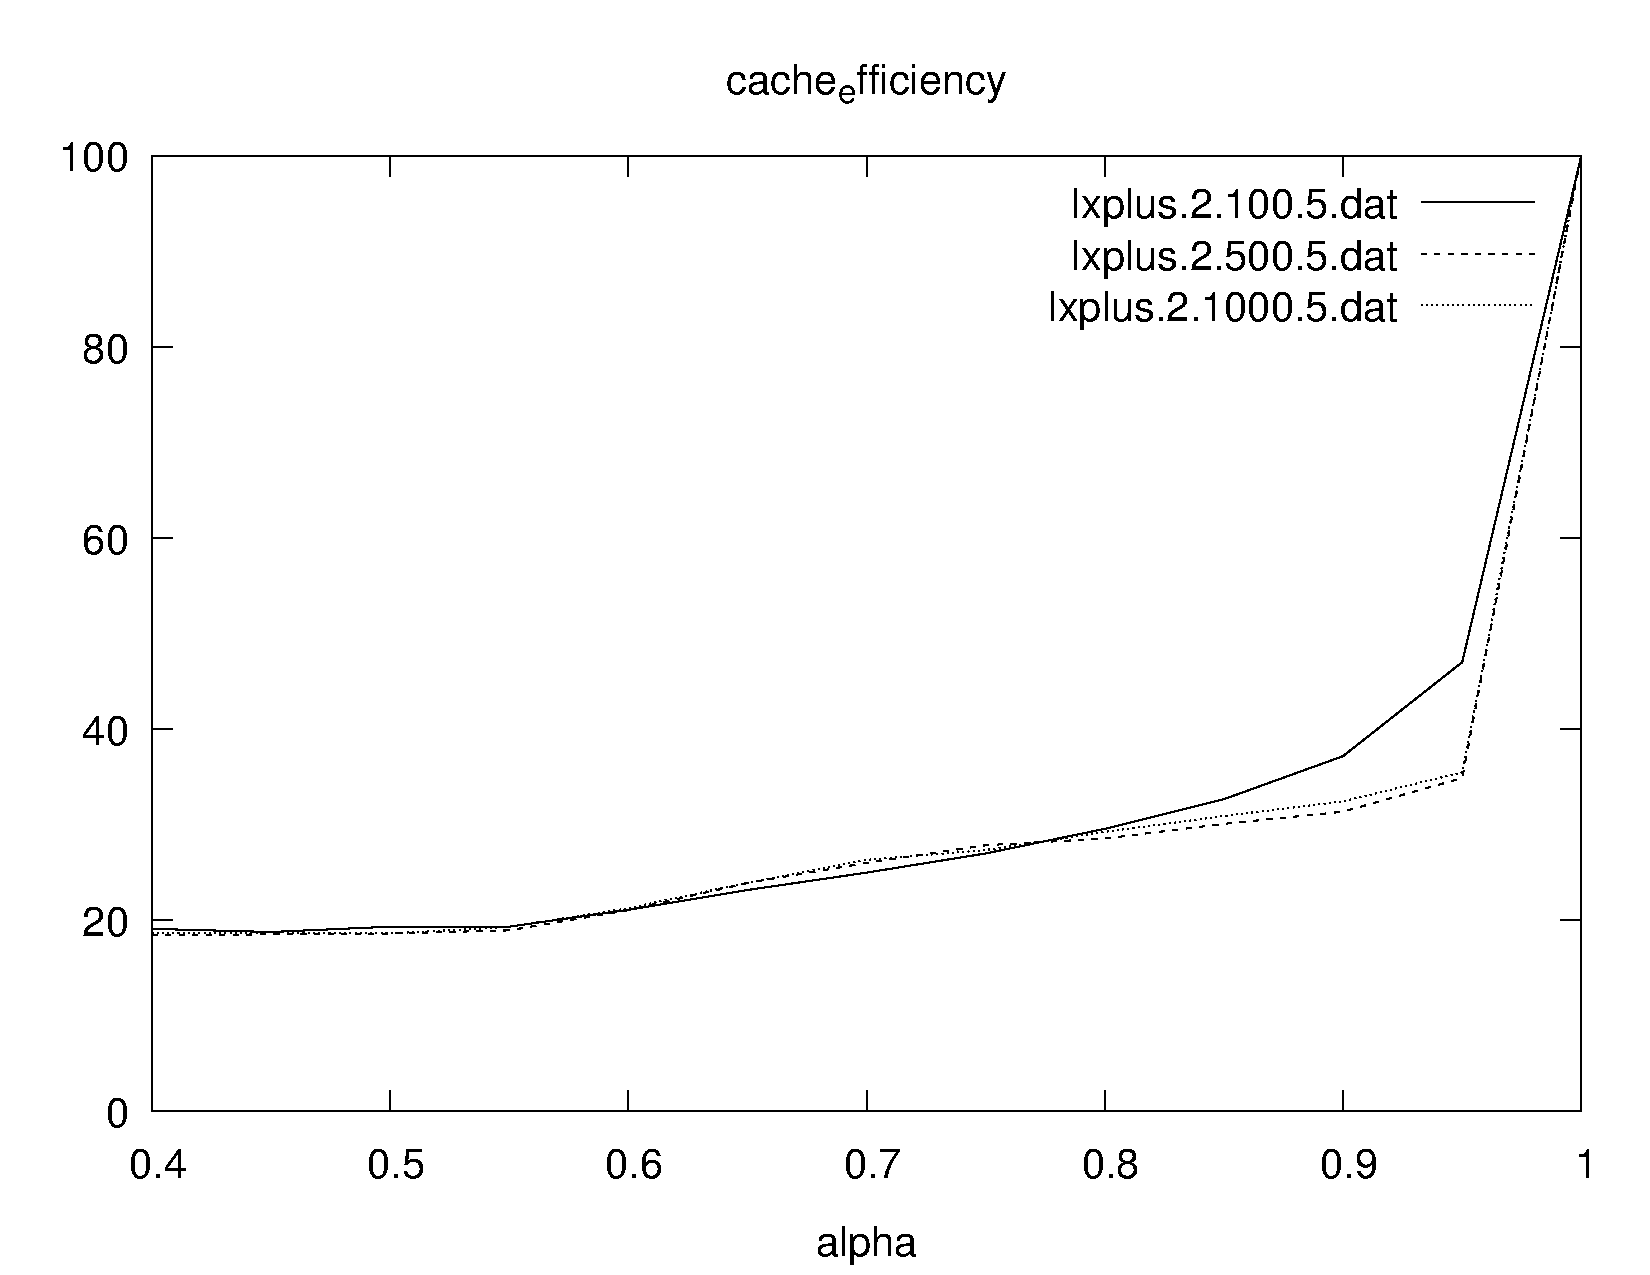
\includegraphics[width=0.48\linewidth]{curated/sensitivity/cache_efficiency_request_percent_plt.pdf}
\caption{}
\end{figure*}

\section{Reproducibility Data}

In an effort to provide consistent, reproducible results outlined are the
resources utilized in this paper and where they can be found.
Specific commits are mentioned to provide the exact version that was used.


All of these repositories are open source and contain Makefiles
and instructions on how to build and run them.

\section*{Acknowledgment}


\bibliographystyle{ACM-Reference-Format}
\bibliography{otherpapers,cclpapers}

\end{document}
